% Chapter 2

\chapter{Quantum Operations} % Main chapter title

\label{Chapter2}

\section{Basic operations}
\label{chapter:basic_opterations}

Before creating a quantum circuit, a basic understanding of quantum operations and gates is needed. Comparable to the classical bit, qubits are the more powerful quantum equivalent. Whilst classical bits can only assume a state of $1$ and $0$, a qubit can be $1$, $0$ or anything in between. The state of a single, non-entangled qubit can be visualized with the Bloch sphere\cite{bloch_nuclear_induction}. Figure \ref{fig:circuit_empty} shows a simple circuit containing one qubit, annotated with $q_0$, and figure \ref{fig:circuit_empty_bloch_sphere} shows the Bloch sphere for it.

\begin{figure}[!h]
    \centering
    \scalebox{1.0}{
        \Qcircuit @C=1.0em @R=1.0em @!R { 
            \nghost{ {q}_{0} :  } & \lstick{ {q}_{0} :  } & \qw & \qw\\ 
        }
    }
    \caption{Quantum circuit with a single qubit and no quantum gates}
    \label{fig:circuit_empty}
\end{figure}

\begin{figure}[!h]
    \centering
    \scalebox{0.3}{
        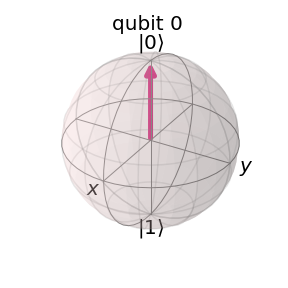
\includegraphics{Appendices/chapter_2/basic_bloch_sphere.png}
    }
    \caption{Bloch sphere with the state $\ket{0}$}
    \label{fig:circuit_empty_bloch_sphere}
\end{figure}

The visible arrow shows the current state, which lies directly on the $z$ axis. The state of the qubit is described as a vector in equation \ref{equation:single_qubit_zero_state}.

\begin{equation}
    \ket{0} = \begin{pmatrix}1 \\ 0\end{pmatrix}
    \label{equation:single_qubit_zero_state}
\end{equation}

The classical NOT gate, that inverts the state of a chosen bit, also exists as a quantum gate. The matrix definition of the Pauli $\mathrm{X}$\cite{qiskit_xgate_nodate} gate is represented in figure \ref{fig:matrix_pauli_x}. When applying it to a qubit, a multiplication of the state vector of $q_0$ and the matrix $\mathrm{X}$ results in the inverted state $\ket{1}$, as demonstrated in equation \ref{equation:pauli_x_example}. The circuit for this example is shown in figure \ref{fig:circuit_negated_empty}. Figure \ref{fig:circuit_negated_empty_bloch_sphere} shows that our state now points in the opposite direction when compared to figure \ref{fig:circuit_empty_bloch_sphere}.

\begin{figure}
    \centering
    $\mathrm{X} = \begin{pmatrix}
        0 & 1 \\
        1 & 0
    \end{pmatrix}$
    \caption{Matrix that defines the Pauli $\mathrm{X}$ gate}
    \label{fig:matrix_pauli_x}
\end{figure}

\begin{figure}[!h]
    \centering
    \scalebox{1.0}{
        \Qcircuit @C=1.0em @R=1.0em @!R { 
            \nghost{ {q}_{0} :  } & \lstick{ {q}_{0} :  } & \gate{\mathrm{X}} & \qw & \qw\\ 
        }
    }
    \caption{Quantum circuit with a single qubit and $\mathrm{X}$ gate}
    \label{fig:circuit_negated_empty}
\end{figure}

\begin{figure}[!h]
    \centering
    \scalebox{0.3}{
        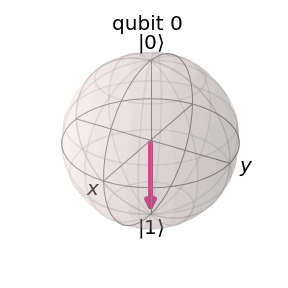
\includegraphics{Appendices/chapter_2/negated_bloch_sphere.png}
    }
    \caption{Bloch sphere with the state $\ket{1}$}
    \label{fig:circuit_negated_empty_bloch_sphere}
\end{figure}

\begin{equation}
    \centering
    \begin{split}
        \mathrm{X}\ket{0} =\ \begin{pmatrix} 0 & 1 \\ 1 & 0 \end{pmatrix}\begin{pmatrix}1 \\ 0\end{pmatrix} =\ \begin{pmatrix}0 \\ 1\end{pmatrix} =\ \ket{1}
    \end{split}
    \label{equation:pauli_x_example}
\end{equation}

A superposition is any state that is neither $\ket{0}$ and $\ket{1}$, but a combination of both. Such a state is defined as $\alpha\ket{0} + \beta\ket{1}$, where the quadratic value of $\alpha$ and $\beta$\footnote{Gross simplification, see chapter \ref{chapter:measurement}} corresponds to the probability of the given state, and therefore $\alpha^2 + \beta^2 = 1$. When building a quantum circuit, the Hadamard, or $\mathrm{H}$\cite{qiskit_hgate_nodate}, gate can be used to put a qubit in an \emph{equal} superposition, that is equal probability for $\ket{0}$ and $\ket{1}$. Figure \ref{fig:matrix_hadamard} shows the matrix definition of the Hadamard gate, figure \ref{fig:circuit_hadamard} a simple single qubit circuit with the Hadamard gate, and equation \ref{equation:hadamard_example} the calculation of said circuit. The Bloch sphere in figure \ref{fig:circuit_hadamard_bloch_sphere} shows the attained superposition, which is orthogonal to the $Z$ axis.

\begin{figure}[!h]
    \centering
    $\mathrm{H} = \frac{1}{\sqrt{2}}\begin{pmatrix}1 & 1 \\1 & -1\end{pmatrix}$
    \caption{Matrix that defines the Hadamard gate}
    \label{fig:matrix_hadamard}
\end{figure}

\begin{equation}
    \centering
    \begin{split}
        \mathrm{H}\ket{0} =\ \frac{1}{\sqrt{2}}\begin{pmatrix}1 & 1 \\1 & -1\end{pmatrix}\begin{pmatrix}1 \\ 0\end{pmatrix} =\ \frac{\ket{0} + \ket{1}}{\sqrt{2}} =\ \frac{1}{\sqrt{2}}\ket{0} + \frac{1}{\sqrt{2}}\ket{1}
    \end{split}
    \label{equation:hadamard_example}
\end{equation}


\begin{figure}[!h]
    \centering
    \scalebox{1.0}{
        \Qcircuit @C=1.0em @R=1.0em @!R { 
            \nghost{ {q}_{0} :  } & \lstick{ {q}_{0} :  } & \gate{\mathrm{H}} & \qw & \qw\\ 
        }
    }
    \caption{Quantum circuit with a single qubit and Hadamard gate}
    \label{fig:circuit_hadamard}
\end{figure}

\begin{figure}[!h]
    \centering
    \scalebox{0.3}{
        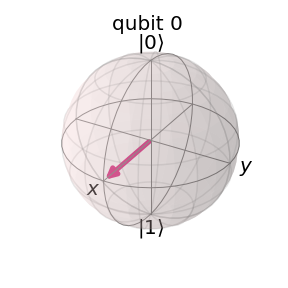
\includegraphics{Appendices/chapter_2/hadamard_bloch_sphere.png}
    }
    \caption{Bloch sphere with the equal superposition state $\frac{1}{\sqrt{2}}\ket{0} + \frac{1}{\sqrt{2}}\ket{1}$}
    \label{fig:circuit_hadamard_bloch_sphere}
\end{figure}

\clearpage

\section{Rotations}
\label{chapter:rotations}

As seen in chapter \ref{chapter:basic_opterations}, quantum gates apply rotations to the state inside the Bloch sphere. There exist parametrizable, rotational gates that rotate the state around a given axis, by the supplied value. One of those gates is the $\mathrm{RY}(\theta)$\cite{qiskit_rygate_nodate} gate. The $\mathrm{RY}$ gate is constructed from the Pauli $\mathrm{Y}$ gate as shown in equation \ref{equation:pauli_y_to_ry}. Note that the resulting power series is equal to the ones defined for $\cos$ and $\sin$ in equation \ref{equation:power_series_sin_cos}\cite{lars_complex_1978}. As measurements in a quantum circuit are, to put it simply, collapsing the state vector onto the $Z$ axis\cite{feynman_feynman_1965}, rotation around the $Y$ axis have a direct impact on the probabilities of the measurement.

\begin{equation}
    \begin{split}
        \mathrm{RY}(\theta) &=\ e^{-i\frac{\theta}{2}\mathrm{Y}} =\ e^{\frac{-i\theta}{2}\begin{pmatrix} 0 & -i \\ i & 0 \end{pmatrix}} \\
        \mathrm{Y}' &=\ -i\frac{\theta}{2}\mathrm{Y} =\ \begin{pmatrix}
                                                         0 & \frac{-\theta}{2}\\
                                                         \frac{\theta}{2} & 0\\
                                                    \end{pmatrix} \\
        e^{\mathrm{Y}'} &=\ I^{2\times2} + \mathrm{Y}' + \frac{\mathrm{Y}'^2}{2!} + \frac{\mathrm{Y}'^3}{3!} + \frac{\mathrm{Y}'^4}{4!} + \cdot\cdot\cdot \\
        \mathrm{RY}(\theta) &=\ \begin{pmatrix}
         1 - \frac{\theta^2}{8} + \frac{\theta^4}{384} + \cdot\cdot\cdot & - \frac{\theta}{2} + \frac{\theta^3}{48} - \frac{\theta^5}{3840} + \cdot\cdot\cdot\\
         \frac{\theta}{2} - \frac{\theta^3}{48} + \frac{\theta^5}{3840} + \cdot\cdot\cdot & 1 - \frac{\theta^2}{8} + \frac{\theta^4}{384} + \cdot\cdot\cdot \\
         \end{pmatrix}\\ &=\ \begin{pmatrix}
        \cos{\frac{\theta}{2}} & -\sin{\frac{\theta}{2}} \\
        \sin{\frac{\theta}{2}} & \cos{\frac{\theta}{2}}
    \end{pmatrix}
    \end{split}
    \label{equation:pauli_y_to_ry}
\end{equation}

\begin{equation}
    \begin{split}
        \cos(x) &=\ 1 - \frac{x^2}{2!} + \frac{x^4}{4!} - \frac{x^6}{6!} + \cdot\cdot\cdot \\
        \sin(x) &= x - \frac{x^3}{3!} + \frac{x^5}{5!} - \frac{x^7}{7!} + \cdot\cdot\cdot
    \end{split}
    \label{equation:power_series_sin_cos}
\end{equation}

\begin{figure}[!h]
    \centering
    \scalebox{1.0}{
        \Qcircuit @C=1.0em @R=1.0em @!R { 
            \nghost{ {q}_{0} :  } & \lstick{ {q}_{0} :  } & \gate{\mathrm{R_Y}\,(\frac{\pi}{2})} & \qw & \qw\\ 
        }
    }
    \caption{Quantum circuit with a single qubit and $\mathrm{RY}$ gate parameterized to $\frac{\pi}{2}$}
    \label{fig:circuit_ry}
\end{figure}

\begin{figure}[!h]
    \centering
    \scalebox{0.3}{
        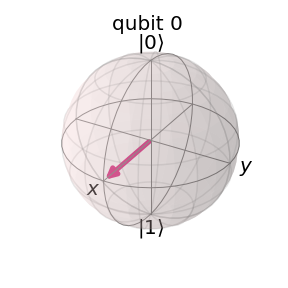
\includegraphics{Appendices/chapter_2/halfpi_yrotation_bloch_sphere.png}
    }
    \caption{Bloch sphere with the equal superposition state $\cos(\frac\pi{4})\ket{0} + \sin(\frac\pi{4})\ket{1}$}
    \label{fig:ry_bloch_sphere}
\end{figure}

\begin{figure}[!h]
    \centering
    \scalebox{0.5}{
        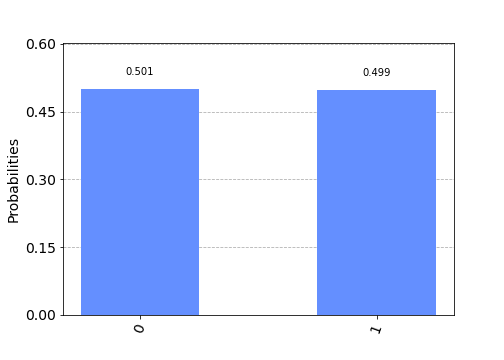
\includegraphics{Appendices/chapter_2/halfpi_yrotation_histogram.png}
    }
    \caption{Histogram of the resulting probabilities for $\ket{0}$ and $\ket{1}$ on circuit \ref{fig:circuit_ry}}
    \label{fig:histogram_ry}
\end{figure}

Quantum circuits with more than one qubit can use the entanglement of multiple qubits for advanced unitary operations. When entangling two qubits together, one has to start with calculating the tensor product of their state vectors. For circuit \ref{fig:circuit_double_hadamard}, the calculations are outlined in equation \ref{equation:two_hadamard_example}.

\begin{figure}[!h]
    \centering
    \scalebox{1.0}{
        \Qcircuit @C=1.0em @R=1.0em @!R { 
            \nghost{ {q}_{0} :  } & \lstick{ {q}_{0} :  } & \gate{\mathrm{H}} & \qw & \qw\\ 
            \nghost{ {q}_{1} :  } & \lstick{ {q}_{1} :  } & \gate{\mathrm{H}} & \qw & \qw\\ 
        }
    }
    \caption{Quantum circuit with two qubits and two Hadamard gates}
    \label{fig:circuit_double_hadamard}
\end{figure}

\begin{equation}
    \centering
    \begin{split}
        \mathrm{H}\ket{0} &=\ \frac{1}{\sqrt{2}}\begin{pmatrix}1 & 1 \\1 & -1\end{pmatrix}\begin{pmatrix}1 \\ 0\end{pmatrix} =\ \frac{\ket{0} + \ket{1}}{\sqrt{2}} \\
        \vec{s} &= \begin{pmatrix}\frac{1}{\sqrt{2}}\\\frac{1}{\sqrt{2}}\end{pmatrix} \otimes \begin{pmatrix}\frac{1}{\sqrt{2}}\\\frac{1}{\sqrt{2}}\end{pmatrix} = \begin{pmatrix}
            \frac{1}{2}\\\frac{1}{2}\\\frac{1}{2}\\\frac{1}{2}
        \end{pmatrix}
    \end{split}
    \label{equation:two_hadamard_example}
\end{equation}

\newpage
Quantum gates can be of any size and use as many qubits as they're designed for. Gates such as $\mathrm{CY}$\cite{qiskit_cygate_nodate}, $\mathrm{CX}$\cite{qiskit_cxgate_nodate} and $\mathrm{CZ}$\cite{qiskit_czgate_nodate} cover two qubits, of which one is a \emph{control} qubit. Depending on its state, the rotation is then applied to the second qubit. Figures \ref{fig:cy_entanglement}, \ref{fig:cx_entanglement} and \ref{fig:cz_entanglement} show the circuit design and the corresponding equations \ref{equation:cy_entanglement}, \ref{equation:cx_entanglement} and \ref{equation:cz_entanglement} show the behaviour of the state vector when entanglement is applied.

%--------------------------------

\begin{figure}[!h]
    \centering
    \scalebox{1.0}{
        \Qcircuit @C=1.0em @R=1.0em @!R { 
            \nghost{ {q}_{0} :  } & \lstick{ {q}_{0} :  } & \gate{\mathrm{H}} & \ctrl{1} & \qw & \qw\\
            \nghost{ {q}_{1} :  } & \lstick{ {q}_{1} :  } & \gate{\mathrm{H}} & \gate{\mathrm{Y}} & \qw & \qw\\
        }
    }
    \caption{Quantum circuit with two qubits, two Hadamard gates and entangled with a $\mathrm{CY}$ gate}
    \label{fig:cy_entanglement}
\end{figure}


\begin{equation}
    \centering
    \begin{split}
        \vec{s}_{\mathrm{CY}} &=\ \mathrm{CY}\begin{pmatrix}
            \frac{1}{2}\\\frac{1}{2}\\\frac{1}{2}\\\frac{1}{2}
        \end{pmatrix} =\  \begin{pmatrix}
        1 & 0 & 0 & 0 \\
        0 & 0 & 0 & -i \\
        0 & 0 & 1 & 0 \\
        0 & i & 0 & 0
    \end{pmatrix}\begin{pmatrix}
            \frac{1}{2}\\\frac{1}{2}\\\frac{1}{2}\\\frac{1}{2}
        \end{pmatrix} \\
        \vec{s}_{\mathrm{CY}} &= \begin{pmatrix}
            \frac{1}{2}\\\frac{-i}{2}\\\frac{1}{2}\\\frac{i}{2}
        \end{pmatrix}
    \end{split}
    \label{equation:cy_entanglement}
\end{equation}

%---------------------------------------

\begin{figure}[!h]
    \centering
    \scalebox{1.0}{
        \Qcircuit @C=1.0em @R=1.0em @!R { 
            \nghost{ {q}_{0} :  } & \lstick{ {q}_{0} :  } & \gate{\mathrm{H}} & \ctrl{1} & \qw & \qw\\
            \nghost{ {q}_{1} :  } & \lstick{ {q}_{1} :  } & \gate{\mathrm{H}} & \gate{\mathrm{X}} & \qw & \qw\\
        }
    }
    \caption{Quantum circuit with two qubits, two Hadamard gates and entangled with a $\mathrm{CX}$ gate}
    \label{fig:cx_entanglement}
\end{figure}

\begin{equation}
    \centering
    \begin{split}
        \vec{s}_{\mathrm{CX}} &=\ \mathrm{CX}\begin{pmatrix}
            \frac{1}{2}\\\frac{1}{2}\\\frac{1}{2}\\\frac{1}{2}
        \end{pmatrix} =\  \begin{pmatrix}
        1 & 0 & 0 & 0 \\
        0 & 0 & 0 & 1 \\
        0 & 0 & 1 & 0 \\
        0 & 1 & 0 & 0
    \end{pmatrix}\begin{pmatrix}
            \frac{1}{2}\\\frac{1}{2}\\\frac{1}{2}\\\frac{1}{2}
        \end{pmatrix} \\
        \vec{s}_{\mathrm{CX}} &= \begin{pmatrix}
            \frac{1}{2}\\\frac{1}{2}\\\frac{1}{2}\\\frac{1}{2}
        \end{pmatrix}
    \end{split}
    \label{equation:cx_entanglement}
\end{equation}

%-----------------------------------

\begin{figure}[!h]
    \centering
    \scalebox{1.0}{
        \Qcircuit @C=1.0em @R=1.0em @!R {
            \nghost{ {q}_{0} :  } & \lstick{ {q}_{0} :  } & \gate{\mathrm{H}} & \ctrl{1} & \qw & \qw\\
            \nghost{ {q}_{1} :  } & \lstick{ {q}_{1} :  } & \gate{\mathrm{H}} & \control\qw & \qw & \qw\\
        }
    }
    \caption{Quantum circuit with two qubits, two Hadamard gates and entangled with a $\mathrm{CZ}$ gate}
    \label{fig:cz_entanglement}
\end{figure}

\begin{equation}
    \centering
    \begin{split}
        \vec{s}_{\mathrm{CZ}} &=\ \mathrm{CZ}\begin{pmatrix}
            \frac{1}{2}\\\frac{1}{2}\\\frac{1}{2}\\\frac{1}{2}
        \end{pmatrix} =\  \begin{pmatrix}
        1 & 0 & 0 & 0 \\
        0 & 1 & 0 & 0 \\
        0 & 0 & 1 & 0 \\
        0 & 0 & 0 & -1
    \end{pmatrix}\begin{pmatrix}
            \frac{1}{2}\\\frac{1}{2}\\\frac{1}{2}\\\frac{1}{2}
        \end{pmatrix} \\
        \vec{s}_{\mathrm{CZ}} &= \begin{pmatrix}
            \frac{1}{2}\\\frac{1}{2}\\\frac{1}{2}\\\frac{-1}{2}
        \end{pmatrix}
    \end{split}
    \label{equation:cz_entanglement}
\end{equation}

\subsection{Measurement}
\label{chapter:measurement}
The statement in chapter \ref{chapter:basic_opterations} of $\alpha^2 + \beta^2 = 1$ is a gross simplification of the  measurement process. When measuring a quantum circuit, it always returns one of all the possible values. This is why, when determining it, multiples \emph{shots} are executed until the achieved distribution of values converges onto their probabilities. This also applies when calculating the probabilities. Whilst it is not necessary to do multiple calculations for each state, each state does need to be calculated separately. To measure the probability of $01$ in a two qubit circuit, we have to use a measurement matrix and surround it with our state $\ket{\psi}$\footnote{$\ket{\psi}$ stands for any arbitrary qubit state} and $\bra{\psi}$, which is the Hermitian transposition\cite{marshall_c_methods_1964} of $\ket{\psi}$. Equation \ref{equation:probability_calculation_example_1} demonstrates the steps needed to measure the probability of state $01$ and equation \ref{equation:probability_calculation_example_2} for state $11$. Further calculations in this chapter will use $M$ to resemble all four, single calculations and show them as a single vector.

\begin{equation}
    \centering
    \begin{split}
        \mathrm{P}_{Example} =\ \bra{\psi}M_2\ket{\psi} =\ \begin{pmatrix}
        \frac{-i}{\sqrt{2}} & \frac{i}{\sqrt{2}} & \frac{-i}{\sqrt{2}} & \frac{-i}{\sqrt{2}}
        \end{pmatrix}\begin{pmatrix}
        0 & 0 & 0 & 0 \\ 
        0 & 1 & 0 & 0 \\ 
        0 & 0 & 0 & 0\\ 
        0 & 0 & 0& 0\end{pmatrix}\begin{pmatrix}
        \frac{i}{\sqrt{2}} \\ \frac{-i}{\sqrt{2}} \\ \frac{i}{\sqrt{2}} \\ \frac{i}{\sqrt{2}}
        \end{pmatrix} =\ \frac{1}{2}
    \end{split}
    \label{equation:probability_calculation_example_1}
\end{equation}

\begin{equation}
    \centering
    \begin{split}
        \mathrm{P}_{Example} =\ \bra{\psi}M_4\ket{\psi} =\ \begin{pmatrix}
        \frac{-i}{\sqrt{2}} & \frac{i}{\sqrt{2}} & \frac{-i}{\sqrt{2}} & \frac{-i}{\sqrt{2}}
        \end{pmatrix}\begin{pmatrix}
        0 & 0 & 0 & 0 \\ 
        0 & 0 & 0 & 0 \\ 
        0 & 0 & 0 & 0\\ 
        0 & 0 & 0& 1\end{pmatrix}\begin{pmatrix}
        \frac{i}{\sqrt{2}} \\ \frac{-i}{\sqrt{2}} \\ \frac{i}{\sqrt{2}} \\ \frac{i}{\sqrt{2}}
        \end{pmatrix} =\ \frac{1}{2}
    \end{split}
    \label{equation:probability_calculation_example_2}
\end{equation}

As entanglement connects both qubits, any gate that is applied to one of those is directly applied to the other one. The circuit \ref{fig:circuit_cz_entangled_ry_gate} shows the $\mathrm{RY}$ gate, parameterized to $\frac{\pi}{4}$,  after the entanglement. To calculate this quantum circuit, an increase in dimensionality of the target gate is done. Equation \ref{equation:2_x_2_ry} demonstrates how the identity matrix is used on the $\mathrm{RY}$ gate.

 \begin{equation}
     \centering
     \begin{split}
        \mathrm{RY}(\theta)^{2\times2} =\ I^{2\times2}\otimes\mathrm{RY}(\theta) =\  \begin{pmatrix}
        \cos{\frac{\theta}{2}} & -\sin{\frac{\theta}{2}} & 0 & 0\\
        \sin{\frac{\theta}{2}} & \cos{\frac{\theta}{2}} & 0 & 0 \\
        0 & 0 & \cos{\frac{\theta}{2}} & -\sin{\frac{\theta}{2}}\\
        0 & 0 & \sin{\frac{\theta}{2}} & \cos{\frac{\theta}{2}}\\
    \end{pmatrix}\\
     \end{split}
     \label{equation:2_x_2_ry}
 \end{equation}

Equations \ref{equation:cz_entanglement_with_ry}, \ref{equation:cx_entanglement_with_ry} and \ref{equation:cy_entanglement_with_ry} show the calculations of the resulting probabilities for each type of entanglement.

\begin{figure}[!ht]
    \centering
    \scalebox{1.0}{
        \Qcircuit @C=1.0em @R=0.2em @!R { 
            \nghost{ {q}_{0} :  } & \lstick{ {q}_{0} :  } & \gate{\mathrm{H}} & \ctrl{1} & \gate{\mathrm{R_Y}\,(\frac{\pi}{4})} & \qw & \qw\\
            \nghost{ {q}_{1} :  } & \lstick{ {q}_{1} :  } & \gate{\mathrm{H}} & \control\qw & \qw & \qw & \qw\
            }
        }
    \caption{Quantum circuit with two qubits, two Hadamard gates, entangled with a $\mathrm{CZ}$ gate and a follow-up $\mathrm{RY}$ gate}
    \label{fig:circuit_cz_entangled_ry_gate}
\end{figure}

\begin{equation}
    \centering
    \begin{split}
    \mathrm{RY}(\theta)^{2\times2}\vec{s}_{\mathrm{CZ}} &=\ \begin{pmatrix}
        \cos{\frac{\theta}{2}} & -\sin{\frac{\theta}{2}} & 0 & 0\\
        \sin{\frac{\theta}{2}} & \cos{\frac{\theta}{2}} & 0 & 0 \\
        0 & 0 & \cos{\frac{\theta}{2}} & -\sin{\frac{\theta}{2}}\\
        0 & 0 & \sin{\frac{\theta}{2}} & \cos{\frac{\theta}{2}}
    \end{pmatrix}\begin{pmatrix}
            \frac{1}{2}\\\frac{1}{2}\\\frac{1}{2}\\\frac{-1}{2}
        \end{pmatrix} \\
        \ket{\psi_{CZ}} &= \begin{pmatrix}
     0.2706\\
     0.65328\\
     0.65328\\
     -0.2706\\
     \end{pmatrix} \\
     \mathrm{P_{CZ}} &=\ \bra{\psi_{CZ}}M\ket{\psi_{CZ}} =\ \begin{pmatrix}
     0.073223\\
     0.42678\\
     0.42678\\
     0.073223\\
     \end{pmatrix}
    \end{split}
    \label{equation:cz_entanglement_with_ry}
\end{equation}

\begin{equation}
    \centering
    \begin{split}
         \mathrm{P_{CX}} &=\ \bra{\psi_{CX}}M\ket{\psi_{CX}} \rightarrow \begin{pmatrix}
         0.073223\\
         0.42678\\
         0.073223\\
         0.42678\\
     \end{pmatrix}
    \end{split}
    \label{equation:cx_entanglement_with_ry}
\end{equation}

\begin{equation}
    \centering
    \begin{split}
         \mathrm{P_{CY}} &=\ \bra{\psi_{CY}}M\ket{\psi_{CY}} \rightarrow \begin{pmatrix}
         0.25\\
         0.25\\
         0.25\\
         0.25\\
     \end{pmatrix}
    \end{split}
    \label{equation:cy_entanglement_with_ry}
\end{equation}

To assess the differences between the application of the rotation gate $\mathrm{RY}$ before the entanglement, circuit \ref{fig:circuit_ry_gate_cz_entangled} is calculated. The initial step of applying $\mathrm{RY}(\theta)$ to $q_0$, is demonstrated in equation \ref{equation:hadamard_ry_before_entanglement}.

\begin{figure}[!ht]
    \centering
    \scalebox{1.0}{
        \Qcircuit @C=1.0em @R=0.2em @!R { 
	 	    \nghost{ {q}_{0} :  } & \lstick{ {q}_{0} :  } & \gate{\mathrm{H}} & \gate{\mathrm{R_Y}\,(\mathrm{\frac{\pi}{4}})} \barrier[0em]{1} & \qw & \ctrl{1} & \qw & \qw\\ 
	 	    \nghost{ {q}_{1} :  } & \lstick{ {q}_{1} :  } & \gate{\mathrm{H}} & \qw & \qw & \control\qw & \qw & \qw\\ 
	 	    \nghost{ {text} :  } & \lstick{  } & & &\ket{\psi_0} & & &\\ 
        }
    }
    \caption{Quantum circuit with two qubits, two Hadamard gates, single $\mathrm{RY}$ gate and entangled with a $\mathrm{CZ}$ gate}
    \label{fig:circuit_ry_gate_cz_entangled}
\end{figure}

\begin{equation}
        \centering
    \begin{split}
          \ket{\psi_0} =\ \mathrm{RY}(\frac{\pi}{4})\mathrm{H}\ket{0} &=\ \begin{pmatrix}
        \cos{\frac{\pi}{8}} & -\sin{\frac{\pi}{8}} \\
        \sin{\frac{\pi}{8}} & \cos{\frac{\pi}{8}}
    \end{pmatrix}\begin{pmatrix}\frac{1}{\sqrt{2}}\\\frac{1}{\sqrt{2}}\end{pmatrix} \\
    \ket{\psi_0} &=\ \begin{pmatrix}
     0.38268\\
     0.92388\\
     \end{pmatrix}
    \end{split}
    \label{equation:hadamard_ry_before_entanglement}
\end{equation}

\begin{equation}
    \centering
    \begin{split}
    \ket{\psi_{CZ}} &=\ \mathrm{CZ}\ket{\psi_0}\otimes\mathrm{H}\ket{0} =\ \begin{pmatrix}
     0.2706\\
     0.2706\\
     0.65328\\
     0.65328\\
     \end{pmatrix} \\
         \mathrm{P_{CZ}} &=\ \bra{\psi_{CZ}}M\ket{\psi_{CZ}} \rightarrow \begin{pmatrix}
         0.073223\\
         0.073223\\
         0.42678\\
         0.42678\\
     \end{pmatrix}
    \end{split}
    \label{equation:h_ry_cz_entanglement}
\end{equation}

\begin{equation}
    \centering
    \begin{split}
    \ket{\psi_{CX}} &=\ \mathrm{CX}\ket{\psi_0}\otimes\mathrm{H}\ket{0} =\ \begin{pmatrix}
     0.2706\\
     0.2706\\
     0.65328\\
     0.65328\\
     \end{pmatrix} \\
    \mathrm{P_{CX}} &=\ \bra{\psi_{CX}}M\ket{\psi_{CX}} \rightarrow \begin{pmatrix}
     0.073223\\
     0.073223\\
     0.42678\\
     0.42678\\
     \end{pmatrix}
    \end{split}
    \label{equation:h_ry_cx_entanglement}
\end{equation}

\begin{equation}
    \centering
    \begin{split}
    \ket{\psi_{CY}} &=\ \mathrm{CY}\ket{\psi_0}\otimes\mathrm{H}\ket{0} =\ \begin{pmatrix}
     0.2706\\
     0-0.65328i\\
     0.65328\\
     0+0.2706i\\
     \end{pmatrix} \\
    \mathrm{P_{CY}} &=\ \bra{\psi_{CY}}M\ket{\psi_{CY}} \rightarrow \begin{pmatrix}
    0.0732\\
    0.4268\\
    0.4268\\
    0.0732\\
     \end{pmatrix}
    \end{split}
    \label{equation:h_ry_cy_entanglement}
\end{equation}

Whereas equation \ref{equation:cy_entanglement_with_ry} shows that when applying $\mathrm{RY}$ after the entanglement, it returns the states to their previous probabilities, equation \ref{equation:h_ry_cy_entanglement} losses none of its operations. This indicates that applying the weights before the entanglement can result in a wider range of results, which \emph{could} lead to a more powerful classifier.

%----------------------------------------------------------------------------------------
\clearpage
\section{Visual Comparison Between A Neural Network And Quantum Circuit}

To design the quantum equivalent to a neural net, a visual comparison is created and traced. Figure \ref{fig:comparison_neuron_feature_weight_quantum} contains an exemplary neural network, where each $\sum_i$ represents a single node. The highlighted paths are converted into their quantum counterparts. In an initial step, the input layer with features and weights is created. Equation \ref{equation:quantum_feature_weight} shows the mathematical operation that is executed on a single qubit.

\begin{figure}[!h]
\begin{subfigure}{.5\textwidth}
\centering
  \begin{tikzpicture}[shorten >=1pt,node distance=1.5cm,on grid,auto]
    	\node (0) {\colorbox{yellow}{$i_0$}};
    	\node (1) [below=of 0] {\colorbox{yellow}{$i_1$}};
    	\node (2) [below=of 1] {\colorbox{yellow}{$i_2$}};
    	\node (3) [below=of 2] {\colorbox{yellow}{$i_3$}};
    	\node (4) [right=of 0] {$\sum_0$};
    	\node (5) [right=of 3] {$\sum_1$};
    	\node (6) [right=of 4] {$\sum_2$};
    	\node (7) [right=of 5] {$\sum_3$};
    	\path[->]
    	(0) edge [preaction={draw,yellow,-,double=yellow,double distance=2\pgflinewidth,}] node {\colorbox{yellow}{$\omega_0$}} (4)
    	(1) edge [preaction={draw,yellow,-,double=yellow,double distance=2\pgflinewidth,},bend right=25] node {\colorbox{yellow}{$\omega_1$}} (4)
    	(2) edge [preaction={draw,yellow,-,double=yellow,double distance=2\pgflinewidth,},bend left=25] node {\colorbox{yellow}{$\omega_2$}} (5)
    	(3) edge [preaction={draw,yellow,-,double=yellow,double distance=2\pgflinewidth,}] node {\colorbox{yellow}{$\omega_3$}} (5)
    	(4) edge (6)
    	(4) edge (7)
    	(5) edge (7);
    \end{tikzpicture}
    \caption{Example neural network, with the weighted input connections being highlighted}
\end{subfigure}
\begin{subfigure}{.5\textwidth}
\centering
    \scalebox{1.0}{
        \Qcircuit @C=1.0em @R=0.2em @!R { 
            \nghost{ {q}_{0} :  } & \lstick{ {q}_{0} :  } & \gate{\mathrm{R_Y}\, (\mathrm{i_0})} & \gate{\mathrm{R_Y}\,(\mathrm{w_0})} & \qw & \qw\\
            \nghost{ {q}_{1} :  } & \lstick{ {q}_{1} :  } & \gate{\mathrm{R_Y}\, (\mathrm{i_1})} & \gate{\mathrm{R_Y}\,(\mathrm{w_1})} & \qw & \qw\\
            \nghost{ {q}_{2} :  } & \lstick{ {q}_{2} :  } & \gate{\mathrm{R_Y}\, (\mathrm{i_2})} & \gate{\mathrm{R_Y}\,(\mathrm{w_2})} & \qw & \qw\\
            \nghost{ {q}_{3} :  } & \lstick{ {q}_{3} :  } & \gate{\mathrm{R_Y}\, (\mathrm{i_3})} & \gate{\mathrm{R_Y}\,(\mathrm{w_3})} & \qw & \qw\\
        }
    }
    \caption{Quantum circuit with four qubits and a pair of two $\mathrm{RY}$ gates per qubit, one for the input feature $i_x$ and one for the weight $w_x$}
\end{subfigure}%
\caption{Comparison of neural network and input and weight gates of the quantum circuit}
\label{fig:comparison_neuron_feature_weight_quantum}
\end{figure}

\begin{equation}
    \centering
    \begin{split}
        \mathrm{RY}(\omega_0)\mathrm{RY}(i_0)\ket{0} &=\ \begin{pmatrix}
        \cos{\frac{\omega_0}{2}} & -\sin{\frac{\omega_0}{2}} \\
        \sin{\frac{\omega_0}{2}} & \cos{\frac{\omega_0}{2}}
    \end{pmatrix}\begin{pmatrix}
        \cos{\frac{i_0}{2}} & -\sin{\frac{i_0}{2}} \\
        \sin{\frac{i_0}{2}} & \cos{\frac{i_0}{2}}
    \end{pmatrix} \begin{pmatrix}
        1 \\ 0
    \end{pmatrix}\\ \rightarrow q_0 &=\ \begin{pmatrix}
     \cos\frac{i_{0}}{2}\cos\frac{\omega_{0}}{2} - \sin\frac{i_{0}}{2}\sin\frac{\omega_{0}}{2}\\
     \cos\frac{i_{0}}{2}\sin\frac{\omega_{0}}{2} + \cos\frac{\omega_{0}}{2}\sin\frac{i_{0}}{2}\\
     \end{pmatrix}
    \end{split}
    \label{equation:quantum_feature_weight}
\end{equation}

It is important to note that whilst graphically they appear to do the same, the behaviour is quite different. Where the computational neuron performs classical multiplications, the quantum counterpart operates with rotations, as demonstrated in chapter \ref{chapter:rotations}. The \emph{probability} of a given state is, depending on the rotation, reinforced or weakened.\par

The next step is to rebuild the two partially connected nodes $\sum_0$ and $\sum_1$, as highlighted in figure \ref{fig:comparison_neuron_feature_weight_entanglement_quantum}. Note that we first have to increase the dimension of the state vector by calculating the tensor product of $q_0$ and $q_1$, as seen in equation \ref{equation:tensor_product_two_qubits}. The entanglement itself is calculated in equation \ref{equation:entanglement_calculation} using the $\mathrm{CZ}$ gate.

\clearpage

\begin{figure}[!h]
\begin{subfigure}{.5\textwidth}
\centering
  \begin{tikzpicture}[shorten >=1pt,node distance=1.5cm,on grid,auto]
    	\node (0) {$i_0$};
    	\node (1) [below=of 0] {$i_1$};
    	\node (2) [below=of 1] {$i_2$};
    	\node (3) [below=of 2] {$i_3$};
    	\node (4) [right=of 0] {\colorbox{yellow}{$\sum_0$}};
    	\node (5) [right=of 3] {\colorbox{yellow}{$\sum_1$}};
    	\node (6) [right=of 4] {$\sum_2$};
    	\node (7) [right=of 5] {$\sum_3$};
    	\path[->]
    	(0) edge node {$\omega_0$} (4)
    	(1) edge [bend right=25] node {$\omega_1$} (4)
    	(2) edge [bend left=25] node {$\omega_2$} (5)
    	(3) edge node {$\omega_3$} (5)
    	(4) edge (6)
    	(4) edge (7)
    	(5) edge (7);
    \end{tikzpicture}
    \caption{Example neural network, with the first two nodes highlighted}
\end{subfigure}
\begin{subfigure}{.5\textwidth}
\centering
    \scalebox{1.0}{
    \Qcircuit @C=1.0em @R=0.2em @!R {
        \nghost{ {q}_{0} :  } & \lstick{ {q}_{0} :  } & \gate{\mathrm{R_Y}\,(\mathrm{i_0})} & \gate{\mathrm{R_Y}\,(\mathrm{w_0})} \barrier[0em]{1} & \qw & \ctrl{1} \barrier[0em]{1}& \qw & \qw\\ 
        \nghost{ {q}_{1} :  } & \lstick{ {q}_{1} :  } & \gate{\mathrm{R_Y}\,(\mathrm{i_1})} & \gate{\mathrm{R_Y}\,(\mathrm{w_1})} & \qw & \control\qw & \qw & \qw\\
        \nghost{} & \lstick{} & & & \ket{\psi_0}  & & \ket{\psi_1} &\\
        \nghost{ {q}_{2} :  } & \lstick{ {q}_{2} :  } & \gate{\mathrm{R_Y}\,(\mathrm{i_2})} & \gate{\mathrm{R_Y}\,(\mathrm{w_2})} & \ctrl{1} & \qw & \qw\\
        \nghost{ {q}_{3} :  } & \lstick{ {q}_{3} :  } & \gate{\mathrm{R_Y}\,(\mathrm{i_3})} & \gate{\mathrm{R_Y}\,(\mathrm{w_3})} & \control\qw & \qw & \qw\\
        }
    }
    \caption{Quantum circuit with four qubits, weighted input gates and entanglement between $q_0,q_1$ and $q_2,q_3$}
\end{subfigure}%
\caption{Comparison of the summation nodes of the neural network and their quantum entanglement equivalent.}
\label{fig:comparison_neuron_feature_weight_entanglement_quantum}
\end{figure}


\begin{equation}
    \centering
    \begin{split}
        \ket{\psi_0} &=\ \mathrm{RY}(\omega_0)\mathrm{RY}(i_0) \otimes \mathrm{RY}(\omega_1)\mathrm{RY}(i_1) \\ 
        \ket{\psi_0} &=\ \begin{pmatrix}
            \cos\frac{i_{0}}{2}\cos\frac{\omega_{0}}{2} - \sin\frac{i_{0}}{2}\sin\frac{\omega_{0}}{2}\\
            \cos\frac{i_{0}}{2}\sin\frac{\omega_{0}}{2} + \cos\frac{\omega_{0}}{2}\sin\frac{i_{0}}{2}\\
        \end{pmatrix} \otimes 
        \begin{pmatrix}
            \cos\frac{i_{1}}{2}\cos\frac{\omega_{1}}{2} - \sin\frac{i_{1}}{2}\sin\frac{\omega_{1}}{2}\\
            \cos\frac{i_{1}}{2}\sin\frac{\omega_{1}}{2} + \cos\frac{\omega_{1}}{2}\sin\frac{i_{1}}{2}\\
        \end{pmatrix} \\
        \ket{\psi_0} &=\ \begin{pmatrix}
     (\cos\frac{i_{0}}{2}\cos\frac{\omega_{0}}{2} - \sin\frac{i_{0}}{2}\sin\frac{\omega_{0}}{2})(\cos\frac{i_{1}}{2}\cos\frac{\omega_{1}}{2} - \sin\frac{i_{1}}{2}\sin\frac{\omega_{1}}{2})\\
     (\cos\frac{i_{0}}{2}\cos\frac{\omega_{0}}{2} - \sin\frac{i_{0}}{2}\sin\frac{\omega_{0}}{2})(\cos\frac{i_{1}}{2}\sin\frac{\omega_{1}}{2} + \cos\frac{\omega_{1}}{2}\sin\frac{i_{1}}{2})\\
     (\cos\frac{i_{0}}{2}\sin\frac{\omega_{0}}{2} + \cos\frac{\omega_{0}}{2}\sin\frac{i_{0}}{2})(\cos\frac{i_{1}}{2}\cos\frac{\omega_{1}}{2} - \sin\frac{i_{1}}{2}\sin\frac{\omega_{1}}{2})\\
     (\cos\frac{i_{0}}{2}\sin\frac{\omega_{0}}{2} + \cos\frac{\omega_{0}}{2}\sin\frac{i_{0}}{2})(\cos\frac{i_{1}}{2}\sin\frac{\omega_{1}}{2} + \cos\frac{\omega_{1}}{2}\sin\frac{i_{1}}{2})\\
    \end{pmatrix}
    \end{split}
    \label{equation:tensor_product_two_qubits}
\end{equation}

\begin{equation}
    \centering
    \begin{split}
        \ket{\psi_1} &=\ CZ_{q_0,q_1}\ket{\psi_0} \\ 
        \ket{\psi_1} &=\ \begin{pmatrix}
        1 & 0 & 0 & 0 \\
        0 & 1 & 0 & 0 \\
        0 & 0 & 1 & 0 \\
        0 & 0 & 0 & -1
    \end{pmatrix}\begin{pmatrix}
     (\cos\frac{i_{0}}{2}\cos\frac{\omega_{0}}{2} - \sin\frac{i_{0}}{2}\sin\frac{\omega_{0}}{2})(\cos\frac{i_{1}}{2}\cos\frac{\omega_{1}}{2} - \sin\frac{i_{1}}{2}\sin\frac{\omega_{1}}{2})\\
     (\cos\frac{i_{0}}{2}\cos\frac{\omega_{0}}{2} - \sin\frac{i_{0}}{2}\sin\frac{\omega_{0}}{2})(\cos\frac{i_{1}}{2}\sin\frac{\omega_{1}}{2} + \cos\frac{\omega_{1}}{2}\sin\frac{i_{1}}{2})\\
     (\cos\frac{i_{0}}{2}\sin\frac{\omega_{0}}{2} + \cos\frac{\omega_{0}}{2}\sin\frac{i_{0}}{2})(\cos\frac{i_{1}}{2}\cos\frac{\omega_{1}}{2} - \sin\frac{i_{1}}{2}\sin\frac{\omega_{1}}{2})\\
     (\cos\frac{i_{0}}{2}\sin\frac{\omega_{0}}{2} + \cos\frac{\omega_{0}}{2}\sin\frac{i_{0}}{2})(\cos\frac{i_{1}}{2}\sin\frac{\omega_{1}}{2} + \cos\frac{\omega_{1}}{2}\sin\frac{i_{1}}{2})\\
    \end{pmatrix} \\
    \ket{\psi_1} &=\ \begin{pmatrix}
     (\cos\frac{i_{0}}{2}\cos\frac{\omega_{0}}{2} - \sin\frac{i_{0}}{2}\sin\frac{\omega_{0}}{2})(\cos\frac{i_{1}}{2}\cos\frac{\omega_{1}}{2} - \sin\frac{i_{1}}{2}\sin\frac{\omega_{1}}{2})\\
     (\cos\frac{i_{0}}{2}\cos\frac{\omega_{0}}{2} - \sin\frac{i_{0}}{2}\sin\frac{\omega_{0}}{2})(\cos\frac{i_{1}}{2}\sin\frac{\omega_{1}}{2} + \cos\frac{\omega_{1}}{2}\sin\frac{i_{1}}{2})\\
     (\cos\frac{i_{0}}{2}\sin\frac{\omega_{0}}{2} + \cos\frac{\omega_{0}}{2}\sin\frac{i_{0}}{2})(\cos\frac{i_{1}}{2}\cos\frac{\omega_{1}}{2} - \sin\frac{i_{1}}{2}\sin\frac{\omega_{1}}{2})\\
     -(\cos\frac{i_{0}}{2}\sin\frac{\omega_{0}}{2} + \cos\frac{\omega_{0}}{2}\sin\frac{i_{0}}{2})(\cos\frac{i_{1}}{2}\sin\frac{\omega_{1}}{2} + \cos\frac{\omega_{1}}{2}\sin\frac{i_{1}}{2})\\
     \end{pmatrix}
    \end{split}
    \label{equation:entanglement_calculation}
\end{equation}

\clearpage

At the end of the neural network, we have two more nodes, one of which is fully connected.

\begin{figure}[!h]
\begin{subfigure}{.5\textwidth}
\centering
  \begin{tikzpicture}[shorten >=1pt,node distance=1.5cm,on grid,auto]
    	\node (0) {$i_0$};
    	\node (1) [below=of 0] {$i_1$};
    	\node (2) [below=of 1] {$i_2$};
    	\node (3) [below=of 2] {$i_3$};
    	\node (4) [right=of 0] {$\sum_0$};
    	\node (5) [right=of 3] {$\sum_1$};
    	\node (6) [right=of 4] {$\sum_2$};
    	\node (7) [right=of 5] {$\sum_3$};
    	\path[->]
    	(0) edge node {$\omega_0$} (4)
    	(1) edge [bend right=25] node {$\omega_1$} (4)
    	(2) edge [bend left=25] node {$\omega_2$} (5)
    	(3) edge node {$\omega_3$} (5)
    	(4) edge (6)
    	(4) edge [preaction={draw,yellow,-,double=yellow,double distance=2\pgflinewidth,}] (7)
    	(5) edge (7);
    \end{tikzpicture}
    \caption{Example neural network, with the connection between node $\sum_0$ and $sum_3$ highlighted}
\end{subfigure}
\begin{subfigure}{.5\textwidth}
\centering
    \scalebox{1.0}{
    \Qcircuit @C=1.0em @R=0.2em @!R {
        \nghost{ {q}_{0} :  } & \lstick{ {q}_{0} :  } & \gate{\mathrm{R_Y}\,(\mathrm{i_0})} & \gate{\mathrm{R_Y}\,(\mathrm{w_0})} & \ctrl{1} & \qw &  \qw \barrier[0em]{3} & \qw & \qw\\ 
        \nghost{ {q}_{1} :  } & \lstick{ {q}_{1} :  } & \gate{\mathrm{R_Y}\,(\mathrm{i_1})} & \gate{\mathrm{R_Y}\,(\mathrm{w_1})} & \control\qw & \qw &  \ctrl{1} & \qw & \qw\\
        \nghost{ {q}_{2} :  } & \lstick{ {q}_{2} :  } & \gate{\mathrm{R_Y}\,(\mathrm{i_2})} & \gate{\mathrm{R_Y}\,(\mathrm{w_2})} & \ctrl{1} \barrier[0em]{1} & \qw  & \control\qw & \qw & \qw\\
        \nghost{ {q}_{3} :  } & \lstick{ {q}_{3} :  } & \gate{\mathrm{R_Y}\,(\mathrm{i_3})} & \gate{\mathrm{R_Y}\,(\mathrm{w_3})} & \control\qw & \qw &  \qw & \qw & \qw\\
        \nghost{ } & \lstick{ } & & & & \ket{\psi_2} & & \ket{\psi_3} & \\
        }
    }
    \caption{Quantum circuit with four qubits, weighted input gates and entanglement between $q_0,q_1$ and $q_2,q_3$, and entanglement between $q_{01}$ and $q_{23}$}
\end{subfigure}%
\caption{Overview of the final quantum circuit in comparison to the neural network}
\label{fig:comparison_measurment_layer}
\end{figure}

The shown neural network is designed to illustrate the core problem that entanglement brings. If we are to recreate the network shown in figure \ref{fig:comparison_measurment_layer}, we get full entanglement of all present qubits. Equation \ref{equation:full_entanglement_with_cz} shows the resulting state  $\ket{\psi_3}$. Figure \ref{fig:full_entanglement_networks} shows different neural network designs that lead to the same quantum circuit. Note that one could always measure a part of the circuit, and use that as an input for the next part that is represented in a different quantum circuit. This would allow us to recreate the given neural network fully, but increase complexity substantially, whilst also reducing the amount of transmitted information throughout the complete neural network.
    \begin{equation}
        \centering
        \resizebox{.9\hsize}{!}{
        $$
            \ket{\psi_3} =(I^{4\time4} \otimes CZ)(\ket{\psi_1} \otimes \ket{\psi_2}) =\ \begin{pmatrix}
         (\cos\frac{i_{0}}{2}\cos\frac{\omega_{0}}{2} - \sin\frac{i_{0}}{2}\sin\frac{\omega_{0}}{2})(\cos\frac{i_{1}}{2}\cos\frac{\omega_{1}}{2} - \sin\frac{i_{1}}{2}\sin\frac{\omega_{1}}{2})(\cos\frac{i_{2}}{2}\cos\frac{\omega_{2}}{2} - \sin\frac{i_{2}}{2}\sin\frac{\omega_{2}}{2})(\cos\frac{i_{3}}{2}\cos\frac{\omega_{3}}{2} - \sin\frac{i_{3}}{2}\sin\frac{\omega_{3}}{2})\\
         (\cos\frac{i_{0}}{2}\cos\frac{\omega_{0}}{2} - \sin\frac{i_{0}}{2}\sin\frac{\omega_{0}}{2})(\cos\frac{i_{1}}{2}\cos\frac{\omega_{1}}{2} - \sin\frac{i_{1}}{2}\sin\frac{\omega_{1}}{2})(\cos\frac{i_{2}}{2}\cos\frac{\omega_{2}}{2} - \sin\frac{i_{2}}{2}\sin\frac{\omega_{2}}{2})(\cos\frac{i_{3}}{2}\sin\frac{\omega_{3}}{2} + \cos\frac{\omega_{3}}{2}\sin\frac{i_{3}}{2})\\
         (\cos\frac{i_{0}}{2}\cos\frac{\omega_{0}}{2} - \sin\frac{i_{0}}{2}\sin\frac{\omega_{0}}{2})(\cos\frac{i_{1}}{2}\cos\frac{\omega_{1}}{2} - \sin\frac{i_{1}}{2}\sin\frac{\omega_{1}}{2})(\cos\frac{i_{2}}{2}\sin\frac{\omega_{2}}{2} + \cos\frac{\omega_{2}}{2}\sin\frac{i_{2}}{2})(\cos\frac{i_{3}}{2}\cos\frac{\omega_{3}}{2} - \sin\frac{i_{3}}{2}\sin\frac{\omega_{3}}{2})\\
         (\cos\frac{i_{0}}{2}\cos\frac{\omega_{0}}{2} - \sin\frac{i_{0}}{2}\sin\frac{\omega_{0}}{2})(\cos\frac{i_{1}}{2}\cos\frac{\omega_{1}}{2} - \sin\frac{i_{1}}{2}\sin\frac{\omega_{1}}{2})(\cos\frac{i_{2}}{2}\sin\frac{\omega_{2}}{2} + \cos\frac{\omega_{2}}{2}\sin\frac{i_{2}}{2})(\cos\frac{i_{3}}{2}\sin\frac{\omega_{3}}{2} + \cos\frac{\omega_{3}}{2}\sin\frac{i_{3}}{2})\\
         (\cos\frac{i_{0}}{2}\cos\frac{\omega_{0}}{2} - \sin\frac{i_{0}}{2}\sin\frac{\omega_{0}}{2})(\cos\frac{i_{1}}{2}\sin\frac{\omega_{1}}{2} + \cos\frac{\omega_{1}}{2}\sin\frac{i_{1}}{2})(\cos\frac{i_{2}}{2}\cos\frac{\omega_{2}}{2} - \sin\frac{i_{2}}{2}\sin\frac{\omega_{2}}{2})(\cos\frac{i_{3}}{2}\cos\frac{\omega_{3}}{2} - \sin\frac{i_{3}}{2}\sin\frac{\omega_{3}}{2})\\
         (\cos\frac{i_{0}}{2}\cos\frac{\omega_{0}}{2} - \sin\frac{i_{0}}{2}\sin\frac{\omega_{0}}{2})(\cos\frac{i_{1}}{2}\sin\frac{\omega_{1}}{2} + \cos\frac{\omega_{1}}{2}\sin\frac{i_{1}}{2})(\cos\frac{i_{2}}{2}\cos\frac{\omega_{2}}{2} - \sin\frac{i_{2}}{2}\sin\frac{\omega_{2}}{2})(\cos\frac{i_{3}}{2}\sin\frac{\omega_{3}}{2} + \cos\frac{\omega_{3}}{2}\sin\frac{i_{3}}{2})\\
         (\cos\frac{i_{0}}{2}\cos\frac{\omega_{0}}{2} - \sin\frac{i_{0}}{2}\sin\frac{\omega_{0}}{2})(\cos\frac{i_{1}}{2}\sin\frac{\omega_{1}}{2} + \cos\frac{\omega_{1}}{2}\sin\frac{i_{1}}{2})(\cos\frac{i_{2}}{2}\sin\frac{\omega_{2}}{2} + \cos\frac{\omega_{2}}{2}\sin\frac{i_{2}}{2})(\cos\frac{i_{3}}{2}\cos\frac{\omega_{3}}{2} - \sin\frac{i_{3}}{2}\sin\frac{\omega_{3}}{2})\\
         (\cos\frac{i_{0}}{2}\cos\frac{\omega_{0}}{2} - \sin\frac{i_{0}}{2}\sin\frac{\omega_{0}}{2})(\cos\frac{i_{1}}{2}\sin\frac{\omega_{1}}{2} + \cos\frac{\omega_{1}}{2}\sin\frac{i_{1}}{2})(\cos\frac{i_{2}}{2}\sin\frac{\omega_{2}}{2} + \cos\frac{\omega_{2}}{2}\sin\frac{i_{2}}{2})(\cos\frac{i_{3}}{2}\sin\frac{\omega_{3}}{2} + \cos\frac{\omega_{3}}{2}\sin\frac{i_{3}}{2})\\
         (\cos\frac{i_{0}}{2}\sin\frac{\omega_{0}}{2} + \cos\frac{\omega_{0}}{2}\sin\frac{i_{0}}{2})(\cos\frac{i_{1}}{2}\cos\frac{\omega_{1}}{2} - \sin\frac{i_{1}}{2}\sin\frac{\omega_{1}}{2})(\cos\frac{i_{2}}{2}\cos\frac{\omega_{2}}{2} - \sin\frac{i_{2}}{2}\sin\frac{\omega_{2}}{2})(\cos\frac{i_{3}}{2}\cos\frac{\omega_{3}}{2} - \sin\frac{i_{3}}{2}\sin\frac{\omega_{3}}{2})\\
         (\cos\frac{i_{0}}{2}\sin\frac{\omega_{0}}{2} + \cos\frac{\omega_{0}}{2}\sin\frac{i_{0}}{2})(\cos\frac{i_{1}}{2}\cos\frac{\omega_{1}}{2} - \sin\frac{i_{1}}{2}\sin\frac{\omega_{1}}{2})(\cos\frac{i_{2}}{2}\cos\frac{\omega_{2}}{2} - \sin\frac{i_{2}}{2}\sin\frac{\omega_{2}}{2})(\cos\frac{i_{3}}{2}\sin\frac{\omega_{3}}{2} + \cos\frac{\omega_{3}}{2}\sin\frac{i_{3}}{2})\\
         (\cos\frac{i_{0}}{2}\sin\frac{\omega_{0}}{2} + \cos\frac{\omega_{0}}{2}\sin\frac{i_{0}}{2})(\cos\frac{i_{1}}{2}\cos\frac{\omega_{1}}{2} - \sin\frac{i_{1}}{2}\sin\frac{\omega_{1}}{2})(\cos\frac{i_{2}}{2}\sin\frac{\omega_{2}}{2} + \cos\frac{\omega_{2}}{2}\sin\frac{i_{2}}{2})(\cos\frac{i_{3}}{2}\cos\frac{\omega_{3}}{2} - \sin\frac{i_{3}}{2}\sin\frac{\omega_{3}}{2})\\
         (\cos\frac{i_{0}}{2}\sin\frac{\omega_{0}}{2} + \cos\frac{\omega_{0}}{2}\sin\frac{i_{0}}{2})(\cos\frac{i_{1}}{2}\cos\frac{\omega_{1}}{2} - \sin\frac{i_{1}}{2}\sin\frac{\omega_{1}}{2})(\cos\frac{i_{2}}{2}\sin\frac{\omega_{2}}{2} + \cos\frac{\omega_{2}}{2}\sin\frac{i_{2}}{2})(\cos\frac{i_{3}}{2}\sin\frac{\omega_{3}}{2} + \cos\frac{\omega_{3}}{2}\sin\frac{i_{3}}{2})\\
         -(\cos\frac{i_{0}}{2}\sin\frac{\omega_{0}}{2} + \cos\frac{\omega_{0}}{2}\sin\frac{i_{0}}{2})(\cos\frac{i_{1}}{2}\sin\frac{\omega_{1}}{2} + \cos\frac{\omega_{1}}{2}\sin\frac{i_{1}}{2})(\cos\frac{i_{2}}{2}\cos\frac{\omega_{2}}{2} - \sin\frac{i_{2}}{2}\sin\frac{\omega_{2}}{2})(\cos\frac{i_{3}}{2}\cos\frac{\omega_{3}}{2} - \sin\frac{i_{3}}{2}\sin\frac{\omega_{3}}{2})\\
         -(\cos\frac{i_{0}}{2}\sin\frac{\omega_{0}}{2} + \cos\frac{\omega_{0}}{2}\sin\frac{i_{0}}{2})(\cos\frac{i_{1}}{2}\sin\frac{\omega_{1}}{2} + \cos\frac{\omega_{1}}{2}\sin\frac{i_{1}}{2})(\cos\frac{i_{2}}{2}\cos\frac{\omega_{2}}{2} - \sin\frac{i_{2}}{2}\sin\frac{\omega_{2}}{2})(\cos\frac{i_{3}}{2}\sin\frac{\omega_{3}}{2} + \cos\frac{\omega_{3}}{2}\sin\frac{i_{3}}{2})\\
         -(\cos\frac{i_{0}}{2}\sin\frac{\omega_{0}}{2} + \cos\frac{\omega_{0}}{2}\sin\frac{i_{0}}{2})(\cos\frac{i_{1}}{2}\sin\frac{\omega_{1}}{2} + \cos\frac{\omega_{1}}{2}\sin\frac{i_{1}}{2})(\cos\frac{i_{2}}{2}\sin\frac{\omega_{2}}{2} + \cos\frac{\omega_{2}}{2}\sin\frac{i_{2}}{2})(\cos\frac{i_{3}}{2}\cos\frac{\omega_{3}}{2} - \sin\frac{i_{3}}{2}\sin\frac{\omega_{3}}{2})\\
         -(\cos\frac{i_{0}}{2}\sin\frac{\omega_{0}}{2} + \cos\frac{\omega_{0}}{2}\sin\frac{i_{0}}{2})(\cos\frac{i_{1}}{2}\sin\frac{\omega_{1}}{2} + \cos\frac{\omega_{1}}{2}\sin\frac{i_{1}}{2})(\cos\frac{i_{2}}{2}\sin\frac{\omega_{2}}{2} + \cos\frac{\omega_{2}}{2}\sin\frac{i_{2}}{2})(\cos\frac{i_{3}}{2}\sin\frac{\omega_{3}}{2} + \cos\frac{\omega_{3}}{2}\sin\frac{i_{3}}{2})\\
         \end{pmatrix}
         $$
        }
        \label{equation:full_entanglement_with_cz}
    \end{equation}

\begin{figure}[!h]
\begin{subfigure}{.5\textwidth}
\centering
  \begin{tikzpicture}[shorten >=1pt,node distance=1.5cm,on grid,auto]
    	\node (0) {$i_0$};
    	\node (1) [below=of 0] {$i_1$};
    	\node (2) [below=of 1] {$i_2$};
    	\node (3) [below=of 2] {$i_3$};
    	\node (4) [right=of 0] {$\sum_0$};
    	\node (5) [right=of 3] {$\sum_1$};
    	\node (6) [right=of 4] {$\sum_2$};
    	\node (7) [right=of 5] {$\sum_3$};
    	\path[->]
    	(0) edge node {$\omega_0$} (4)
    	(1) edge [bend right=25] node {$\omega_1$} (4)
    	(2) edge [bend left=25] node {$\omega_2$} (5)
    	(3) edge node {$\omega_3$} (5)
    	(4) edge (6)
    	(5) edge (6)
    	(5) edge (7);
    \end{tikzpicture}
\end{subfigure}
\begin{subfigure}{.5\textwidth}
\centering
  \begin{tikzpicture}[shorten >=1pt,node distance=1.5cm,on grid,auto]
    	\node (0) {$i_0$};
    	\node (1) [below=of 0] {$i_1$};
    	\node (2) [below=of 1] {$i_2$};
    	\node (3) [below=of 2] {$i_3$};
    	\node (4) [right=of 0] {$\sum_0$};
    	\node (5) [right=of 3] {$\sum_1$};
    	\node (6) [right=of 4] {$\sum_2$};
    	\node (7) [right=of 5] {$\sum_3$};
    	\path[->]
    	(0) edge node {$\omega_0$} (4)
    	(1) edge [bend right=25] node {$\omega_1$} (4)
    	(2) edge [bend left=25] node {$\omega_2$} (5)
    	(3) edge node {$\omega_3$} (5)
    	(4) edge (6)
    	(4) edge (7)
    	(5) edge (6)
    	(5) edge (7);
    \end{tikzpicture}
\end{subfigure}%
\caption{Example neural networks that all lead to the same quantum circuit illustrated in figure \ref{fig:comparison_neuron_feature_weight_entanglement_quantum}}
\label{fig:full_entanglement_networks}
\end{figure}